\documentclass[border=4pt,12pt]{standalone}
% House style for redrawn exam diagrams (diagram-v4: 0.4pt lines, filled -latex arrows, fine dashes; stipple and hatching drawn as real dots/lines (no PDF/SVG patterns, so they render in every browser and at any scale); transparent background). Every figure \input's this.
\usepackage{amsmath,amssymb}
\usepackage{txfonts}
\usepackage{pdfrender,xcolor}
% \halo{text}: label on shading. The shading stops just around each letter's outline (a thin knock-out that follows the
% glyphs, like the papers' typesetting), never a box. Owner: "I don't want a box around the text".
\newcommand{\halo}[1]{\leavevmode\rlap{\pdfrender{TextRenderingMode=2,LineWidth=2.2pt,LineJoinStyle=1,StrokeColor=white,FillColor=white}#1}#1}
\usepackage{tikz,pgfplots}
\pgfplotsset{compat=1.18}
\usetikzlibrary{arrows.meta,calc,angles,quotes,patterns,patterns.meta,intersections,positioning,decorations.markings,shapes.geometric}
% Stipple and hatching are drawn as actual dots / lines clipped to the region (path picture), NOT as pattern fills:
% SVG <pattern> fills vanish or blur when browsers scale the image, so the owner could not see the shading.
% Each dot is a 0.72pt square (keeps SVGs small; reads as a dot at print size). Dots sit on one global staggered grid, so neighbouring regions line up.
\makeatletter
\newdimen\ex@x \newdimen\ex@y \newdimen\ex@xa \newdimen\ex@ya \newdimen\ex@xb \newdimen\ex@yb \newcount\ex@row
\def\exam@stipplecolor{black!75}\def\exam@dotr{0.42pt}\def\exam@dotgap{2.5}
\def\ex@rowdots{\ifdim\ex@x<\ex@xb \pgfpathrectangle{\pgfqpoint{\dimexpr\ex@x-0.36pt\relax}{\dimexpr\ex@y-0.36pt\relax}}{\pgfqpoint{0.72pt}{0.72pt}}\advance\ex@x by \exam@dotgap pt\relax\expandafter\ex@rowdots\fi}
\def\exam@stipple{%
  \pgftransformreset% dots are sized in real points even inside scaled pictures
  \pgfpointanchor{path picture bounding box}{south west}\ex@xa=\pgf@x \ex@ya=\pgf@y
  \pgfpointanchor{path picture bounding box}{north east}\ex@xb=\pgf@x \ex@yb=\pgf@y
  \pgfsetfillcolor{\exam@stipplecolor}\pgfmathsetmacro\ex@h{\exam@dotgap/2}%
  \pgfmathtruncatemacro\ex@r{floor(\ex@ya/\ex@h)-1}\ex@row=\ex@r\relax
  \ex@y=\ex@r\dimexpr\ex@h pt\relax
  \loop\ifdim\ex@y<\ex@yb
    \pgfmathtruncatemacro\ex@c{floor(\ex@xa/\exam@dotgap)-1}\ex@x=\ex@c\dimexpr\exam@dotgap pt\relax
    \ifodd\ex@row \advance\ex@x by \ex@h pt\fi
    \ex@rowdots
    \advance\ex@y by \ex@h pt \advance\ex@row by 1
    \ifnum\numexpr\ex@row-(\ex@row/4)*4\relax=0 \pgfusepath{fill}\fi% flush every 4 rows: bounded TeX memory, few clip copies in the SVG
  \repeat\pgfusepath{fill}}
\newdimen\ex@d
\def\exam@hatch#1{% #1 = 1 for /, -1 for \ ; lines 45 degrees, 3pt apart
  \pgftransformreset
  \pgfpointanchor{path picture bounding box}{south west}\ex@xa=\pgf@x \ex@ya=\pgf@y
  \pgfpointanchor{path picture bounding box}{north east}\ex@xb=\pgf@x \ex@yb=\pgf@y
  \ex@d=\dimexpr\ex@yb-\ex@ya\relax \ex@x=\dimexpr\ex@xa-\ex@d\relax
  \loop\ifdim\ex@x<\ex@xb
    \ifnum#1>0 \pgfpathmoveto{\pgfqpoint{\ex@x}{\ex@ya}}\pgfpathlineto{\pgfqpoint{\dimexpr\ex@x+\ex@d\relax}{\ex@yb}}%
    \else \pgfpathmoveto{\pgfqpoint{\ex@x}{\ex@yb}}\pgfpathlineto{\pgfqpoint{\dimexpr\ex@x+\ex@d\relax}{\ex@ya}}\fi
    \advance\ex@x by 4.24pt
  \repeat
  \pgfsetlinewidth{0.4pt}\pgfsetstrokecolor{black}\pgfusepath{stroke}}
\def\examstipple{\exam@stipple}\def\examhatch{\exam@hatch}\def\examsetstipplecolor#1{\def\exam@stipplecolor{#1}}\def\examsetdotgap#1{\def\exam@dotgap{#1}}
\makeatother
% (legacy pattern kept for old files)
% staggered stipple like the NESA papers' dotted shading
\pgfdeclarepatternformonly{exam stipple}{\pgfpointorigin}{\pgfqpoint{2.2pt}{2.2pt}}{\pgfqpoint{2.2pt}{2.2pt}}{%
  \pgfpathcircle{\pgfqpoint{0.55pt}{0.55pt}}{0.42pt}\pgfpathcircle{\pgfqpoint{1.65pt}{1.65pt}}{0.42pt}\pgfusepath{fill}}
\tikzset{
  every picture/.style={line width=0.6pt, >={Latex[length=2mm,width=1.3mm]}},
  curve/.style={line width=0.6pt},
  open arrow/.style={-{Latex[length=2mm,width=1.3mm]}},  % owner: filled -latex heads everywhere, no open chevrons
  aux/.style={dash pattern=on 2pt off 1.5pt, line width=0.6pt},
  shade/.code={\def\exA{#1}\def\exB{none}\ifx\exA\exB\else\pgfkeysalso{fill=black!18}\fi},
  shade/.default=on,
  shade dots/.style={fill=none, path picture={\examstipple}},
  stipple color/.code={\examsetstipplecolor{#1}},
  stipple gap/.code={\examsetdotgap{#1}},
  shade dense dots/.style={fill=none, stipple gap=1.6, path picture={\examstipple}},
  shade hatch/.style={fill=none, path picture={\examhatch{1}}},
  shade hatch reverse/.style={fill=none, path picture={\examhatch{-1}}},
  shade solid/.style={fill=black},
  pt/.style={circle, fill, inner sep=1.1pt},
  open pt/.style={circle, draw, fill=white, inner sep=1.1pt},
}
\pgfplotsset{
  exam axes/.style={axis lines=middle, axis line style={->}, xlabel={$x$}, ylabel={$y$},
    xlabel style={anchor=west}, ylabel style={anchor=south}, tick label style={font=\small},
    every axis plot/.append style={line width=0.6pt, black}, samples=200, clip=false,
    enlargelimits=false, axis on top},
}

\begin{document}
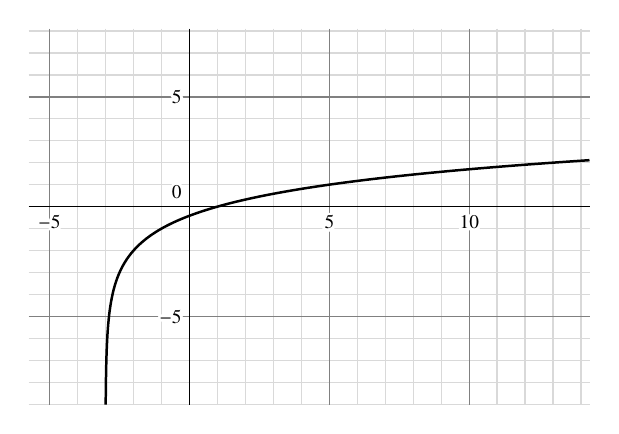
\begin{tikzpicture}[x=0.0127cm, y=-0.0127cm]
  \draw[black!15] (49.00,0.00) -- (49.00,376.20);
  \draw[black!15] (77.00,0.00) -- (77.00,376.20);
  \draw[black!15] (105.00,0.00) -- (105.00,376.20);
  \draw[black!15] (133.00,0.00) -- (133.00,376.20);
  \draw[black!15] (189.00,0.00) -- (189.00,376.20);
  \draw[black!15] (217.00,0.00) -- (217.00,376.20);
  \draw[black!15] (245.00,0.00) -- (245.00,376.20);
  \draw[black!15] (273.00,0.00) -- (273.00,376.20);
  \draw[black!15] (329.00,0.00) -- (329.00,376.20);
  \draw[black!15] (357.00,0.00) -- (357.00,376.20);
  \draw[black!15] (385.00,0.00) -- (385.00,376.20);
  \draw[black!15] (413.00,0.00) -- (413.00,376.20);
  \draw[black!15] (469.00,0.00) -- (469.00,376.20);
  \draw[black!15] (497.00,0.00) -- (497.00,376.20);
  \draw[black!15] (525.00,0.00) -- (525.00,376.20);
  \draw[black!15] (553.00,0.00) -- (553.00,376.20);
  \draw[black!15] (0.00,376.20) -- (561.40,376.20);
  \draw[black!15] (0.00,354.20) -- (561.40,354.20);
  \draw[black!15] (0.00,332.20) -- (561.40,332.20);
  \draw[black!15] (0.00,310.20) -- (561.40,310.20);
  \draw[black!15] (0.00,266.20) -- (561.40,266.20);
  \draw[black!15] (0.00,244.20) -- (561.40,244.20);
  \draw[black!15] (0.00,222.20) -- (561.40,222.20);
  \draw[black!15] (0.00,200.20) -- (561.40,200.20);
  \draw[black!15] (0.00,156.20) -- (561.40,156.20);
  \draw[black!15] (0.00,134.20) -- (561.40,134.20);
  \draw[black!15] (0.00,112.20) -- (561.40,112.20);
  \draw[black!15] (0.00,90.20) -- (561.40,90.20);
  \draw[black!15] (0.00,46.20) -- (561.40,46.20);
  \draw[black!15] (0.00,24.20) -- (561.40,24.20);
  \draw[black!15] (0.00,2.20) -- (561.40,2.20);
  \draw[black!50] (21.00,0.00) -- (21.00,376.20);
  \node[anchor=north,inner sep=0,font=\scriptsize] at (21.00,186.20) {\halo{$-5$}};
  \draw[black!50] (301.00,0.00) -- (301.00,376.20);
  \node[anchor=north,inner sep=0,font=\scriptsize] at (301.00,186.20) {\halo{$5$}};
  \draw[black!50] (441.00,0.00) -- (441.00,376.20);
  \node[anchor=north,inner sep=0,font=\scriptsize] at (441.00,186.20) {\halo{$10$}};
  \draw[black!50] (0.00,288.20) -- (561.40,288.20);
  \node[anchor=east,inner sep=0,font=\scriptsize] at (154.00,288.20) {\halo{$-5$}};
  \draw[black!50] (0.00,68.20) -- (561.40,68.20);
  \node[anchor=east,inner sep=0,font=\scriptsize] at (154.00,68.20) {\halo{$5$}};
  \draw (0.00,178.20) -- (561.40,178.20);
  \draw (161.00,0.00) -- (161.00,376.20);
  \node[anchor=south east,inner sep=0,font=\scriptsize] at (154.00,171.00) {\halo{$0$}};
  \begin{scope}\clip (0.00,0.00) rectangle (561.40,376.20);
  \draw[smooth, line width=0.9pt] plot coordinates {(77.22,376.20) (77.27,369.09) (77.34,362.00) (77.43,354.91) (77.54,347.81) (77.67,340.72) (77.84,333.63) (78.05,326.54) (78.31,319.45) (78.64,312.36) (79.04,305.28) (79.55,298.21) (80.19,291.14) (80.98,284.08) (81.97,277.07) (83.20,270.07) (84.71,263.15) (86.56,256.30) (88.82,249.56) (91.53,243.02) (94.73,236.70) (98.46,230.64) (102.68,224.94) (107.37,219.62) (112.48,214.69) (117.92,210.16) (123.65,206.00) (129.64,202.16) (135.81,198.64) (142.13,195.41) (148.56,192.42) (155.08,189.65) (161.68,187.07) (168.35,184.67) (175.09,182.41) (181.88,180.28) (188.68,178.29) (195.50,176.41) (202.37,174.62) (209.31,172.91) (216.15,171.31) (223.08,169.77) (230.08,168.28) (237.04,166.87) (244.01,165.52) (250.99,164.22) (257.93,162.98) (264.92,161.77) (271.96,160.61) (278.89,159.50) (285.95,158.41) (293.01,157.35) (300.03,156.34) (307.01,155.36) (314.07,154.40) (321.05,153.48) (328.10,152.58) (335.19,151.69) (342.17,150.84) (349.34,150.00) (356.37,149.19) (363.41,148.40) (370.45,147.63) (377.49,146.88) (384.52,146.14) (391.52,145.43) (398.69,144.71) (405.62,144.04) (412.71,143.36) (419.95,142.68) (426.93,142.04) (434.05,141.40) (441.11,140.78) (448.08,140.18) (455.18,139.58) (462.19,138.99) (469.34,138.41) (476.38,137.85) (483.54,137.28) (490.59,136.74) (497.76,136.19) (504.80,135.66) (511.70,135.16) (518.97,134.63) (525.84,134.14) (533.08,133.63) (540.16,133.14) (547.07,132.67) (554.37,132.18) (561.21,131.73)};\end{scope}
\end{tikzpicture}
\end{document}
